\documentclass{beamer}

\usepackage[utf8]{inputenc}
\usepackage{tikz}
\usepackage{natbib}
\usepackage{graphicx}
\usepackage{amsmath}
\usepackage{amssymb}
\usepackage{amsfonts}
%\usepackage{algorithm}
%\usepackage{algorithmic}
\usepackage{setspace}
\usepackage{subfig}
\usepackage{adjustbox}
\usepackage{tikz}

%math fonts
\usefonttheme[onlymath]{serif}

\usetikzlibrary{arrows,automata,positioning}
\usetikzlibrary{shapes.multipart}
\usetikzlibrary{decorations.markings}
\usetikzlibrary{decorations.pathreplacing}

\makeatletter
\def\th@mystyle{
    %\normalfont % body font
    \setbeamercolor{block title example}{bg=myred,fg=white}
    \setbeamercolor{block body example}{bg=lightgray!20,fg=black}
    \def\inserttheoremblockenv{exampleblock}
  }
\makeatother
\theoremstyle{mystyle}
\newtheorem*{remark}{Remark}

\usetheme{metropolis} 
\usecolortheme{beaver}
\fontfamily{verdana}

\definecolor{myred}{HTML}{cc0000}

\setbeamertemplate{itemize item}{\color{myred}\bf{-}}
\setbeamertemplate{itemize subitem}{\color{myred}$\blacktriangleright$}
\setbeamercolor{item in toc}{fg=myred}
\setbeamercolor{title}{fg=black}

\setbeamercolor{frametitle}{fg=myred}
\setbeamerfont{footnote}{size=\tiny}


\usetikzlibrary{arrows,automata,positioning}
\usetikzlibrary{shapes.multipart}
\usetikzlibrary{decorations.markings}
\usetikzlibrary{decorations.pathreplacing}

% macros:
\newcommand{\tS}{\text{t}}   % for terminal states
\newcommand{\cA}{\mathcal{A}}
\newcommand{\cB}{\mathcal{B}}
\newcommand{\cC}{\mathcal{C}}
\newcommand{\cD}{\mathcal{D}}
\newcommand{\cE}{\mathcal{E}}
\newcommand{\cJ}{\mathcal{J}}
\newcommand{\cL}{\mathcal{L}}
\newcommand{\cM}{\mathcal{M}}
\newcommand{\cP}{\mathcal{P}}
\newcommand{\cR}{\mathcal{R}}
\newcommand{\cS}{\mathcal{S}}
\newcommand{\cT}{\mathcal{T}}
\newcommand{\cU}{\mathcal{U}}
\newcommand{\cV}{\mathcal{V}}
\newcommand{\cX}{\mathcal{X}}

\newcommand{\EE}[1]{\mathbb{E}\left[#1\right]}
\newcommand{\EEc}[2]{\mathbb{E}\left[#1\;\middle\lvert\;#2\right]}
\newcommand{\pa}[1]{\left(#1\right)}

\newcommand{\diag}{\text{diag}}
\newcommand{\real}{\mathbb{R}}

\titlegraphic{%
  \hspace{10em}
\includegraphics[width=3cm,height=1.6cm,keepaspectratio]{Figures/upf_logo.png}\hfill
}

\title[Globally Optimal HRL for LMDPs]{Globally Optimal Hierarchical Reinforcement Learning for Linearly-Solvable Markov Decision Processes}
%\subtitle{(Submitted to NeurIPS 2021)}
\author[G. Infante, A. Jonsson, V. Gómez ]{Guillermo Infante, Anders Jonsson, Vicenç Gómez }
\date[July 2021]{July 2021}



\begin{document}

\begin{frame}
   \maketitle
\end{frame}

\begin{frame}{Overview}
\tableofcontents
\end{frame}

\section{Introduction}

\begin{frame}{Introduction}

\begin{itemize}
    \item Hierarchical reinforcement learning (HRL) aims to make learning more efficient by exploiting decomposition in a problem~\cite{conf/nips/Wen20}.
    \item LMDPs are a computationally efficient way to model sequential decision problems~\citep{TodorovNIPS2007}.
    %\item Computing optimal policies for LMDPs is equivalent to a probabilistic inference task~\cite{KappenML2012}.
    \item LMDPs are strongly related to entropy-regularized RL~\cite{optionkeyb} and have been already used in hierarchical settings \cite{saxe2017hierarchy, conf/icaps/Jonsson16}.
    \item Our method presented here retrieves the globally optimal value function efficiently in a hierarchical setting using LMDPs, in contrast to \textit{hierarchically optimal} and \textit{recursively optimal} approaches \cite{dietterich2000hierarchical}.
\end{itemize}
    
\end{frame}


\section{Background}
\begin{frame}{Background - LMDPs (i)}

    An LMDP~\citep{KappenML2012,TodorovNIPS2007} is as a tuple $\cL=\langle\cS,\cT,\cP,\cR,\cJ\rangle$, where:
    
    \begin{itemize}
        \item  $\cS$ is a discrete set of non-terminal states.
        \item $\cT$ is a set of terminal states.
        \item We use $\cS^+=\cS\cup\cT$ to denote the full set of states.
        \item $\cP:\cS\rightarrow\cS^+$ is an uncontrolled transition function.
        \item $\cR:\cS\rightarrow\real$ is a reward function for non-terminal states, assumed to be non-negative.
        \item $\cJ:\cT\rightarrow\real$ is a reward function for terminal states, assumed to be non-negative.

    \end{itemize}
    

  

    The \textbf{learning agent} follows a policy $\pi:\cS\rightarrow\cS^+$, which is a conditional distribution over next states $\pi(\cdot | s_t)$.
\end{frame}


\begin{frame}{Background - LMDPs (ii)}
    
    \begin{itemize}

        \item At time-step $t$ agent receives reward \[ \cR(s_t,\pi) = \cR(s_t) - \lambda\cdot\mathrm{KL}(\pi(\cdot|s_t)\Vert\, \cP(\cdot|s_t)). \]

        \item The aim of the agent is to maximize \[ v^\pi(s) = \EEc{\sum_{t=1}^{T-1} \cR(S_t,\pi) + \cJ(S_T)}{S_1 = s}.\]
        
       \item We obtain the following Bellman optimality equation 
       \begin{align*}
            \frac 1 \lambda v(s) &= \frac 1 \lambda \max_\pi \left[ \cR(s,\pi) + \mathbb{E}_{s'\sim\pi(\cdot|s)} v(s') \right]\\
             &= \frac 1 \lambda \cR(s) + \max_\pi \mathbb{E}_{s'\sim\pi(\cdot|s)} \left[ \frac 1 \lambda v(s') - \log \frac {\pi(s'|s)} {\cP(s'|s)} \right] \;\; (\forall s).
        \end{align*}

    \end{itemize}
\end{frame}

\begin{frame}{Background - LMDPs (iii)}
    
    \begin{itemize}
         \item Taking the exponential transformation $z(s)=e^{v(s)/\lambda}$ for each $s\in\cS^+$ leads to Bellman equations that are linear in $z$ \[ z(s) = e^{\cR(s)/\lambda} \sum_{s'}\cP(s'|s)z(s'). \]
         \item If $\cP$ and $\cR$ are known, this problem can be formulated as an eigenvector problem \[ \mathbf{z} = R P \mathbf{z^+} \text{  where  } R=\text{diag}(e^{\cR(\cdot)/\lambda}) \] where initially 
         $\mathbf z  = \bf 1$.
        \end{itemize}
\end{frame}

\begin{frame}{Background - LMDPs (iii) - online setting}

\begin{itemize}
\item The previous approach requires using the full transition matrix what makes it {\color{blue} intractable} when the state space is large.
\item Alternatively, there exists an online {\color{blue} (corrected)} update rule  
        
         \[ \hat{z}(s_t) \leftarrow (1-\alpha_t) \hat{z}(s_t) + \alpha_t e^{r_t/\lambda}\hat{z}(s_{t+1}) {\color{blue} \frac {\cP(s_{t+1}|s_t)} {\hat{\pi}(s_{t+1}|s_t)}}. \]
         
\item Once $z$ is computed, policies are derived using \[ \pi(s'|s) = \frac {\cP(s'|s)z(s')} {\sum_{s''} \cP(s''|s)z(s'')}\]
    which ...
\end{itemize}
\end{frame}


\begin{frame}{Background - Compositionality}
    \begin{itemize}
    \item Let $\{\cL_1,\ldots,\cL_n\}$ be a collection of LMDPs. 
   
    \item Each LMDP $\cL_i$ only differ in the reward structure of each terminal state $\tS\in\cT$ (i.e. $\cJ_i(\tS)$).
    
    \item Let us consider a new LMDP $\cL$ whose (exponential) reward structure at terminal states can be expressed as follows~\cite{TodorovNIPS2009} 
    \begin{equation*}
        e^{\cJ(\tS)/\lambda} = z(\tS) = \sum_{k=1}^n w_k e^{\cJ_k(\tS)/\lambda}.
    \end{equation*}
    
    \item Since the Bellman equation is linear in $z$, then the optimal value function of any $s \in \cS$ satisfies the same equation above
    
    \begin{equation*}
       z(s) =  \sum_{k=1}^n w_k z_k(s) 
    \end{equation*}
    
    \end{itemize}
    
\end{frame}

\section{Hierarchical LMDPs}
\begin{frame}{Hierarchical LMDPs (i)}

    \begin{itemize}
        \item Hierarchical decomposition nspired by the work of Wen et al.~\cite{conf/nips/Wen20}. 
        \item Given an LMDP $\cL$, its state space $\cS$ is partitioned into $L$ subsets $\{\cS_i\}_{i=1}^L$. 
        \item Each such subset $\cS_i$ induces a subtask, represented by an LMDP $\cL_i=\langle\cS_i,\cT_i,\cP_i,\cR_i,\cJ_i\rangle$:
        \begin{enumerate}
        \item The set of non-terminal states is $\cS_i$.
        \item The set of terminal states $\cT_i$ includes all states in $\cS^+\setminus\cS_i$ that are reachable in one step from a state in $\cS_i$.
        \item $\cP_i:\cS_i\rightarrow\cS_i^+$ and $\cR_i:\cS_i\rightarrow\real$ are restrictions of $\cP$ and $\cR$ to $\cS_i$.
        \item Reward at $\tau\in\cT_i$ equals $\cJ_i(\tau)=\cJ(\tau)$ if $\tau\in\cT$, and $\cJ_i(\tau)=\hat{v}(\tau)$ otherwise, where $\hat{v}(\tau)$ is the estimated value in $\cL$ of the non-terminal state $\tau\in\cS \setminus \cS_i$.
        \end{enumerate}
        
\end{itemize}

\end{frame}

\begin{frame}{Hierarchical LMDPs (ii)}

\begin{definition}
Two subtasks $\cL_i$ and $\cL_j$ are equivalent if there exists a bijection $f:\cS_i\rightarrow\cS_j$ such that the transition probabilities and rewards of non-terminal states are equivalent through $f$.
\end{definition}

\begin{itemize}
    
     
    \item We define a set of {\em exit states} $\cE=\cup_{i=1}^L\cT_i$
    \item We also use $\cE_i=\cE\cap\cS_i$ to denote the set of (non-terminal) exit states in the subtask $\cL_i$. 
    
    \item  A set of equivalence classes $\cC=\{\cC_1,\ldots,\cC_C\}$, $C\leq L$, i.e.~a partition of the set of subtasks $\{\cL_1,\ldots,\cL_L\}$ such that all subtasks in a given partition are equivalent.
    
    \item We represent a single subtask $\cL_j=\langle\cS_j,\cT_j,\cP_j,\cR_j,\cJ_j\rangle$ per equivalence class $\cC_j\in\cC$. 
    
\end{itemize}

    
\end{frame}

\begin{frame}{Example}

\begin{figure}
\begin{center}
\begin{tikzpicture}
\draw[step=0.4,thin,shift={(0.2,0.2)}] (0.8,0.8) grid (4.8,4.8);
\draw[ultra thick] (1,1) rectangle (5,5);
\draw[ultra thick] (3,1) -- (3,1.8);
\draw[ultra thick] (3,2.2) -- (3,3.8);
\draw[ultra thick] (3,4.2) -- (3,5);
\draw[ultra thick] (1,3) -- (1.8,3);
\draw[ultra thick] (2.2,3) -- (3.8,3);
\draw[ultra thick] (4.2,3) -- (5,3);

\draw[fill] (0.6,1.8) rectangle (1,2.2);
\draw[fill] (0.6,3.8) rectangle (1,4.2);
\draw[fill] (1.8,5) rectangle (2.2,5.4);
\draw[fill] (1.8,0.6) rectangle (2.2,1);
\draw[fill] (3.8,0.6) rectangle (4.2,1);
\draw[fill] (5,1.8) rectangle (5.4,2.2);
\draw[fill] (5,3.8) rectangle (5.4,4.2);
\draw[fill] (3.8,5) rectangle (4.2,5.4);

\draw[fill] (2.2,2.2) rectangle (2.6,2.6);
\draw[fill] (4.2,2.2) rectangle (4.6,2.6);
\draw[fill] (2.2,4.2) rectangle (2.6,4.6);


\draw[ultra thick] (4.2,4.2) rectangle (4.6,4.6);
\draw[ultra thick] (3.8,2.6) rectangle (4.2,3.4);
\draw[ultra thick] (1.8,2.6) rectangle (2.2,3.4);
\draw[ultra thick] (2.6,3.8) rectangle (3.4,4.2);
\draw[ultra thick] (2.6,1.8) rectangle (3.4,2.2);

\node at (4.4,4.4) {\small $G$};
\node at (2,3.2) {\small $1^B$};
\node at (2,2.8) {\small $2^T$};
\node at (4,3.2) {\small $3^B$};
\node at (4,2.8) {\small $4^T$};
\node at (2.8,4) {\small $1^R$};
\node at (2.8,2) {\small $2^R$};
\node at (3.2,4) {\small $3^L$};
\node at (3.2,2) {\small $4^L$};

\draw[step=0.4,thin,shift={(0.2,0)}] (8.799,1.999) grid (10.8,4);
\draw[ultra thick] (9,3.2) -- (8.6,3.2) -- (8.6,2.8) -- (9,2.8) -- (9,2) -- (9.8,2);
\draw[ultra thick] (9,3.2) -- (9,4) -- (9.8,4) -- (9.8,4.4) -- (10.2,4.4) -- (10.2,4);
\draw[ultra thick] (10.2,4) -- (11,4) -- (11,3.2) -- (11.4,3.2) -- (11.4,2.8) -- (11,2.8);
\draw[ultra thick] (9.8,2) -- (9.8,1.6) -- (10.2,1.6) -- (10.2,2) -- (11,2) -- (11,2.8);
\draw[ultra thick] (10.2,3.2) rectangle (10.6,3.6);

\node at (10.4,3.4) {\small $G$};
\node at (8.8,3)    {\small $L$};
\node at (11.2,3)   {\small $R$};
\node at (10,1.8)   {\small $B$};
\node at (10,4.2)   {\small $T$};

\node at (3,0.7) {a)};
\node at (10,0.7) {b)};
\end{tikzpicture}
\end{center}
\caption{a) A 4-room LMDP, with all exit states highlighted; b) a single subtask with 5 terminal states $G,L,R,T,B$ that is equivalent to all 4 room subtasks.}
\end{figure}

\end{frame}

\section{Subtask compositionality}

\begin{frame}{Subtask compositionality (i)}

\begin{itemize}
    \item For a subtask $\cL_j=\langle\cS_j,\cT_j,\cP_j,\cR_j,\cJ_j\rangle$ as defined previously, consider its terminal set~$\cT_j=\{\tau_1,\ldots,\tau_n\}$.
    \item We define {\color{blue} $n$ base LMDPs} $\cL_j^1,\ldots,\cL_j^n$, where each base LMDP  $\cL_j^k$ only differ in the reward of terminal states $\cJ_j^k$.
    \item Concretely, $z_j^k(\tau)=1$ if $\tau=\tau_k$, and $z_j^k(\tau)=0$ otherwise. This corresponds to an actual reward of $\cJ_j^k(\tau)=0$ for $\tau=\tau_k$, and $\cJ_j^k(\tau)=-\infty$ otherwise.
    \item Thus, we can solve these {\color{blue} base LMDPs} to obtain $z_j^1,\ldots,z_j^n$.
    \item Having an estimate $\hat z(s)$ for each $t \in \cT_j$, then by compositionality
    \begin{equation*}\label{eq:comp}
        \hat{z}(\tau)=\hat{z}(\tau_1)z_j^1(\tau)+\cdots+\hat{z}(\tau_n)z_j^n(\tau)
    \end{equation*}
\end{itemize}

    
\end{frame}


\begin{frame}{Subtask compositionality (ii)}


\begin{itemize}
    \item Thanks to compositionality, the estimated value of each non-terminal state $s\in\cS_i$ is
    \begin{equation*}
        \hat{z}(s)=\hat{z}(\tau_1)z_j^1(s)+\cdots+\hat{z}(\tau_n)z_j^n(s) \;\; \forall s\in\cS_i,\forall\cL_i\in\cC_j.
    \end{equation*}
    
    \item Terminal states $\tau_1 \dots \tau_n$ are by definition in $\cE$.
    
   \item Having access to a value estimate $\hat{z}_\cE:\cE\rightarrow\mathbb{R}$ and the base LMDPs value functions $z_j^1,\ldots,z_j^n$, is enough to express the value estimate of each other state without learning.
   
   \item No need to store an explicit estimate $\hat z(s)$.
   
   \item {\color{blue} Once we have solved the base LMDPs, there is no need to solve again each individual subtask}. That is why we represent a single subtask $\cL_j$ for each equivalence class $\cC_j$.
    
\end{itemize}

\end{frame}


\begin{frame}{Subtask compositionality (iii)}

\begin{remark}[]
    
    If $\hat z(s)$ is optimal for $s \in \cE$, then $\hat z(s)$ for $s \in \cS_i$ will also be optimal. Thanks to compositionality we have \[\hat z(s) = \hat z(1^R) * z_L(s) + \hat z(4^T) * z_B(s) + \hat z(G) * z_G(s)\]
    
    For any state $s$ in $\cS_i$ represented in red. Thus, if $\hat z = z^*$ for terminal states, then it will be optimal for the interior states as well.
    
    
\end{remark}

\begin{figure}
\begin{center}

\scalebox{0.6}{
\begin{tikzpicture}
\draw[step=0.4,thick,shift={(0.2,0.2)}] (0.8,0.8) grid (4.8, 4.8);
\draw[step=0.4,thick,shift={(0.2,0.2)}, color=red] (2.8, 2.8) grid (4.8, 4.8);


\draw[ultra thick] (1,1) rectangle (5,5);
\draw[ultra thick] (3,1) -- (3,1.8);
\draw[ultra thick] (3,2.2) -- (3,3.8);
\draw[ultra thick, color=red] (3,3) -- (3,5);
\draw[ultra thick] (1,3) -- (1.8,3);
\draw[ultra thick] (2.2,3) -- (3.8,3);
\draw[ultra thick, color=red] (3,3) -- (5,3);

\draw[fill] (0.6,1.8) rectangle (1,2.2);
\draw[fill] (0.6,3.8) rectangle (1,4.2);
\draw[fill] (1.8,5) rectangle (2.2,5.4);
\draw[fill] (1.8,0.6) rectangle (2.2,1);
\draw[fill] (3.8,0.6) rectangle (4.2,1);
\draw[fill] (5,1.8) rectangle (5.4,2.2);
\draw[fill, color=red] (5,3.8) rectangle (5.4,4.2);
\draw[fill, color=red] (3.8,5) rectangle (4.2,5.4);

\draw[ultra thick, color=red] (4.2,4.2) rectangle (4.6,4.6);
\draw[ultra thick, color=red] (3.8,2.6) rectangle (4.2,3.4);
\draw[ultra thick] (1.8,2.6) rectangle (2.2,3.4);
\draw[ultra thick, color=red] (2.6,3.8) rectangle (3.4,4.2);
\draw[ultra thick] (2.6,1.8) rectangle (3.4,2.2);

\node at (4.4,4.4) {\small $G$};
\node at (2,3.2) {\small $1^B$};
\node at (2,2.8) {\small $2^T$};
\node at (4,3.2) {\small $3^B$};
\node at (4,2.8) {\small $4^T$};
\node at (2.8,4) {\small $1^R$};
\node at (2.8,2) {\small $2^R$};
\node at (3.2,4) {\small $3^L$};
\node at (3.2,2) {\small $4^L$};

\draw[step=0.4,thin,shift={(0.2,0)}] (8.799,1.999) grid (10.8,4);
\draw[ultra thick] (9,3.2) -- (8.6,3.2) -- (8.6,2.8) -- (9,2.8) -- (9,2) -- (9.8,2);
\draw[ultra thick] (9,3.2) -- (9,4) -- (9.8,4) -- (9.8,4.4) -- (10.2,4.4) -- (10.2,4);
\draw[ultra thick] (10.2,4) -- (11,4) -- (11,3.2) -- (11.4,3.2) -- (11.4,2.8) -- (11,2.8);
\draw[ultra thick] (9.8,2) -- (9.8,1.6) -- (10.2,1.6) -- (10.2,2) -- (11,2) -- (11,2.8);
\draw[ultra thick] (10.2,3.2) rectangle (10.6,3.6);

\node at (10.4,3.4) {\small $G$};
\node at (8.8,3)    {\small $L$};
\node at (11.2,3)   {\small $R$};
\node at (10,1.8)   {\small $B$};
\node at (10,4.2)   {\small $T$};

\end{tikzpicture}
}
\end{center}
\end{figure}
    
\end{frame}

\section{Algorithms}

\begin{frame}{Eigenvector algorithm (i)}
\begin{itemize}
    \item In the case of known dynamics, we can directly solve $\cL_j$ for each equivalence class $\cC_j$.
    \item We can reformulate the system of equations yielded by
    \begin{equation*}
        \hat{z}(s)=\hat{z}(\tau_1) {\color{blue} z_j^1(s)}+\cdots+\hat{z}(\tau_n){\color{blue}z_j^n(s)} \;\; \forall s\in\cS_i,\forall\cL_i\in\cC_j.
    \end{equation*}
    to be defined only in the states $s \in \cE$.
    
    \item Thus, we define 
    
    \begin{equation*}\label{eq:exits}
     {\bf z}_\cE=G{\bf z}_\cE.
    \end{equation*}
    
    \item $G$ contains the value of the base LMDPs, while $\mathbf{z}_\cE$ is initialized with value 1 for all $s \in \cE$.
    \item No need to keep an estimate of the interior states in the higher level, the values for states in $\cE$ are sufficient.
\end{itemize}
    
\end{frame}

\begin{frame}{Eigenvector algorithm (ii) - Convergence proof}

\begin{lemma}[1]
    If the reward of each terminal state $t\in\cT_i$ equals its optimal value in $\cL$, i.e.~$z_i(t)=z(t)$, the optimal value of each non-terminal state $s\in\cS_i$ equals its optimal value in $\cL$, i.e.~$z_i(s)=z(s)$.
\end{lemma}

\begin{lemma}[2]
    The solution to  ${\bf z}_\cE=G{\bf z}_\cE$ is unique.
\end{lemma}
    

\begin{lemma}[3]
    For each subtask $\cL_i$ and state $s\in\cS_i^+$, it holds that $z_i^1(s)+\cdots+z_i^n(s)\leq 1$.
\end{lemma}

\end{frame}

\begin{frame}{Eigenvector algorithm (iii) - Convergence proof}
Extending on previously stated lemmas:
\begin{itemize}
    \item The base case happens at terminal states $t_\ell\in\cT_i$. In such case $z_i^1(t_\ell)+\cdots+z_i^n(t_\ell) = z_i^\ell(t_\ell) = 1$.
    \item The Bellman equation for the base LMDPs is \[
    z_i^1(s)+\cdots+z_i^n(s)=
    {\color{orange} e^{\cR_i(s)/\lambda}}
    \sum_{s'}{\color{red} P(s'|s)}\left[z_i^1(s')+\cdots+z_i^n(s')\right].
    \]

\item ${\color{orange} e^{\cR_i(s)/\lambda} < 1}$ since $\cR_i(s) < 0$ holds.

\item And since $\left[z_i^1(s')+\cdots+z_i^n(s')\right] \leq 1$ also holds, by induction $z_i^1(s)+\cdots+z_i^n(s) \leq 1$.

\item Thus, in the equation\[ z_\cE = G z_\cE \]G has spectral radius at most 1. The power iteration method will find the eigenvector for the the largest eigenvalue 1.



\end{itemize}
    
\end{frame}

\begin{frame}{Online algorithm (i)}

\begin{itemize}
    
    \item In the case of the online algorithm, we keep an estimate of the base value functions $\hat{z}_j^1,\ldots,\hat{z}_j^n$ for each $\cL_j$.
    \item A single transition is enough to update the value functions of all base LMDPs associated with  $\cL_j$ by using intra-task learning \cite{Kaelbling93}.
    \item The update rule for the states in the exit set becomes
    \[
        \hat{z}_\cE(s) \leftarrow (1 - \alpha_\ell) \hat{z}_\cE(s) + \alpha_\ell [\hat{z}_\cE(t_1) {\color{blue}\hat{z}_j^1(s)} + \cdots + \hat{z}_\cE(t_n) {\color{blue} \hat{z}_j^n(s)}].
    \]
    \item Estimates at any level are learned in an episodic fashion.
    \item When to update states in $\cE$ is still a question to answer. We propose the following alternatives (next slide).
\end{itemize}
    
\end{frame}


\begin{frame}{Online algorithm (ii)}

\begin{itemize}
\item[$V_1$:] Update the value of an exit state $s\in\cE_i$ each time we take a transition from $s$.
\item[$V_2$:] When we reach a terminal state of the subtask $\cL_i$, update the values of all exit states in $\cE_i$.
\item[$V_3$:] When we reach a terminal state of the subtask $\cL_i$, update the values of all exit states in $\cE_i$ and all exit states of subtasks in the equivalence class $\cC_j$ of $\cL_i$.
\end{itemize}


    
\end{frame}



\section{Experiments}
\begin{frame}{Experiments - Rooms domain}


\begin{itemize}
    \item We varied the size of the rooms as well as the number of rooms.
\end{itemize}

\begin{figure}[H]
\centering
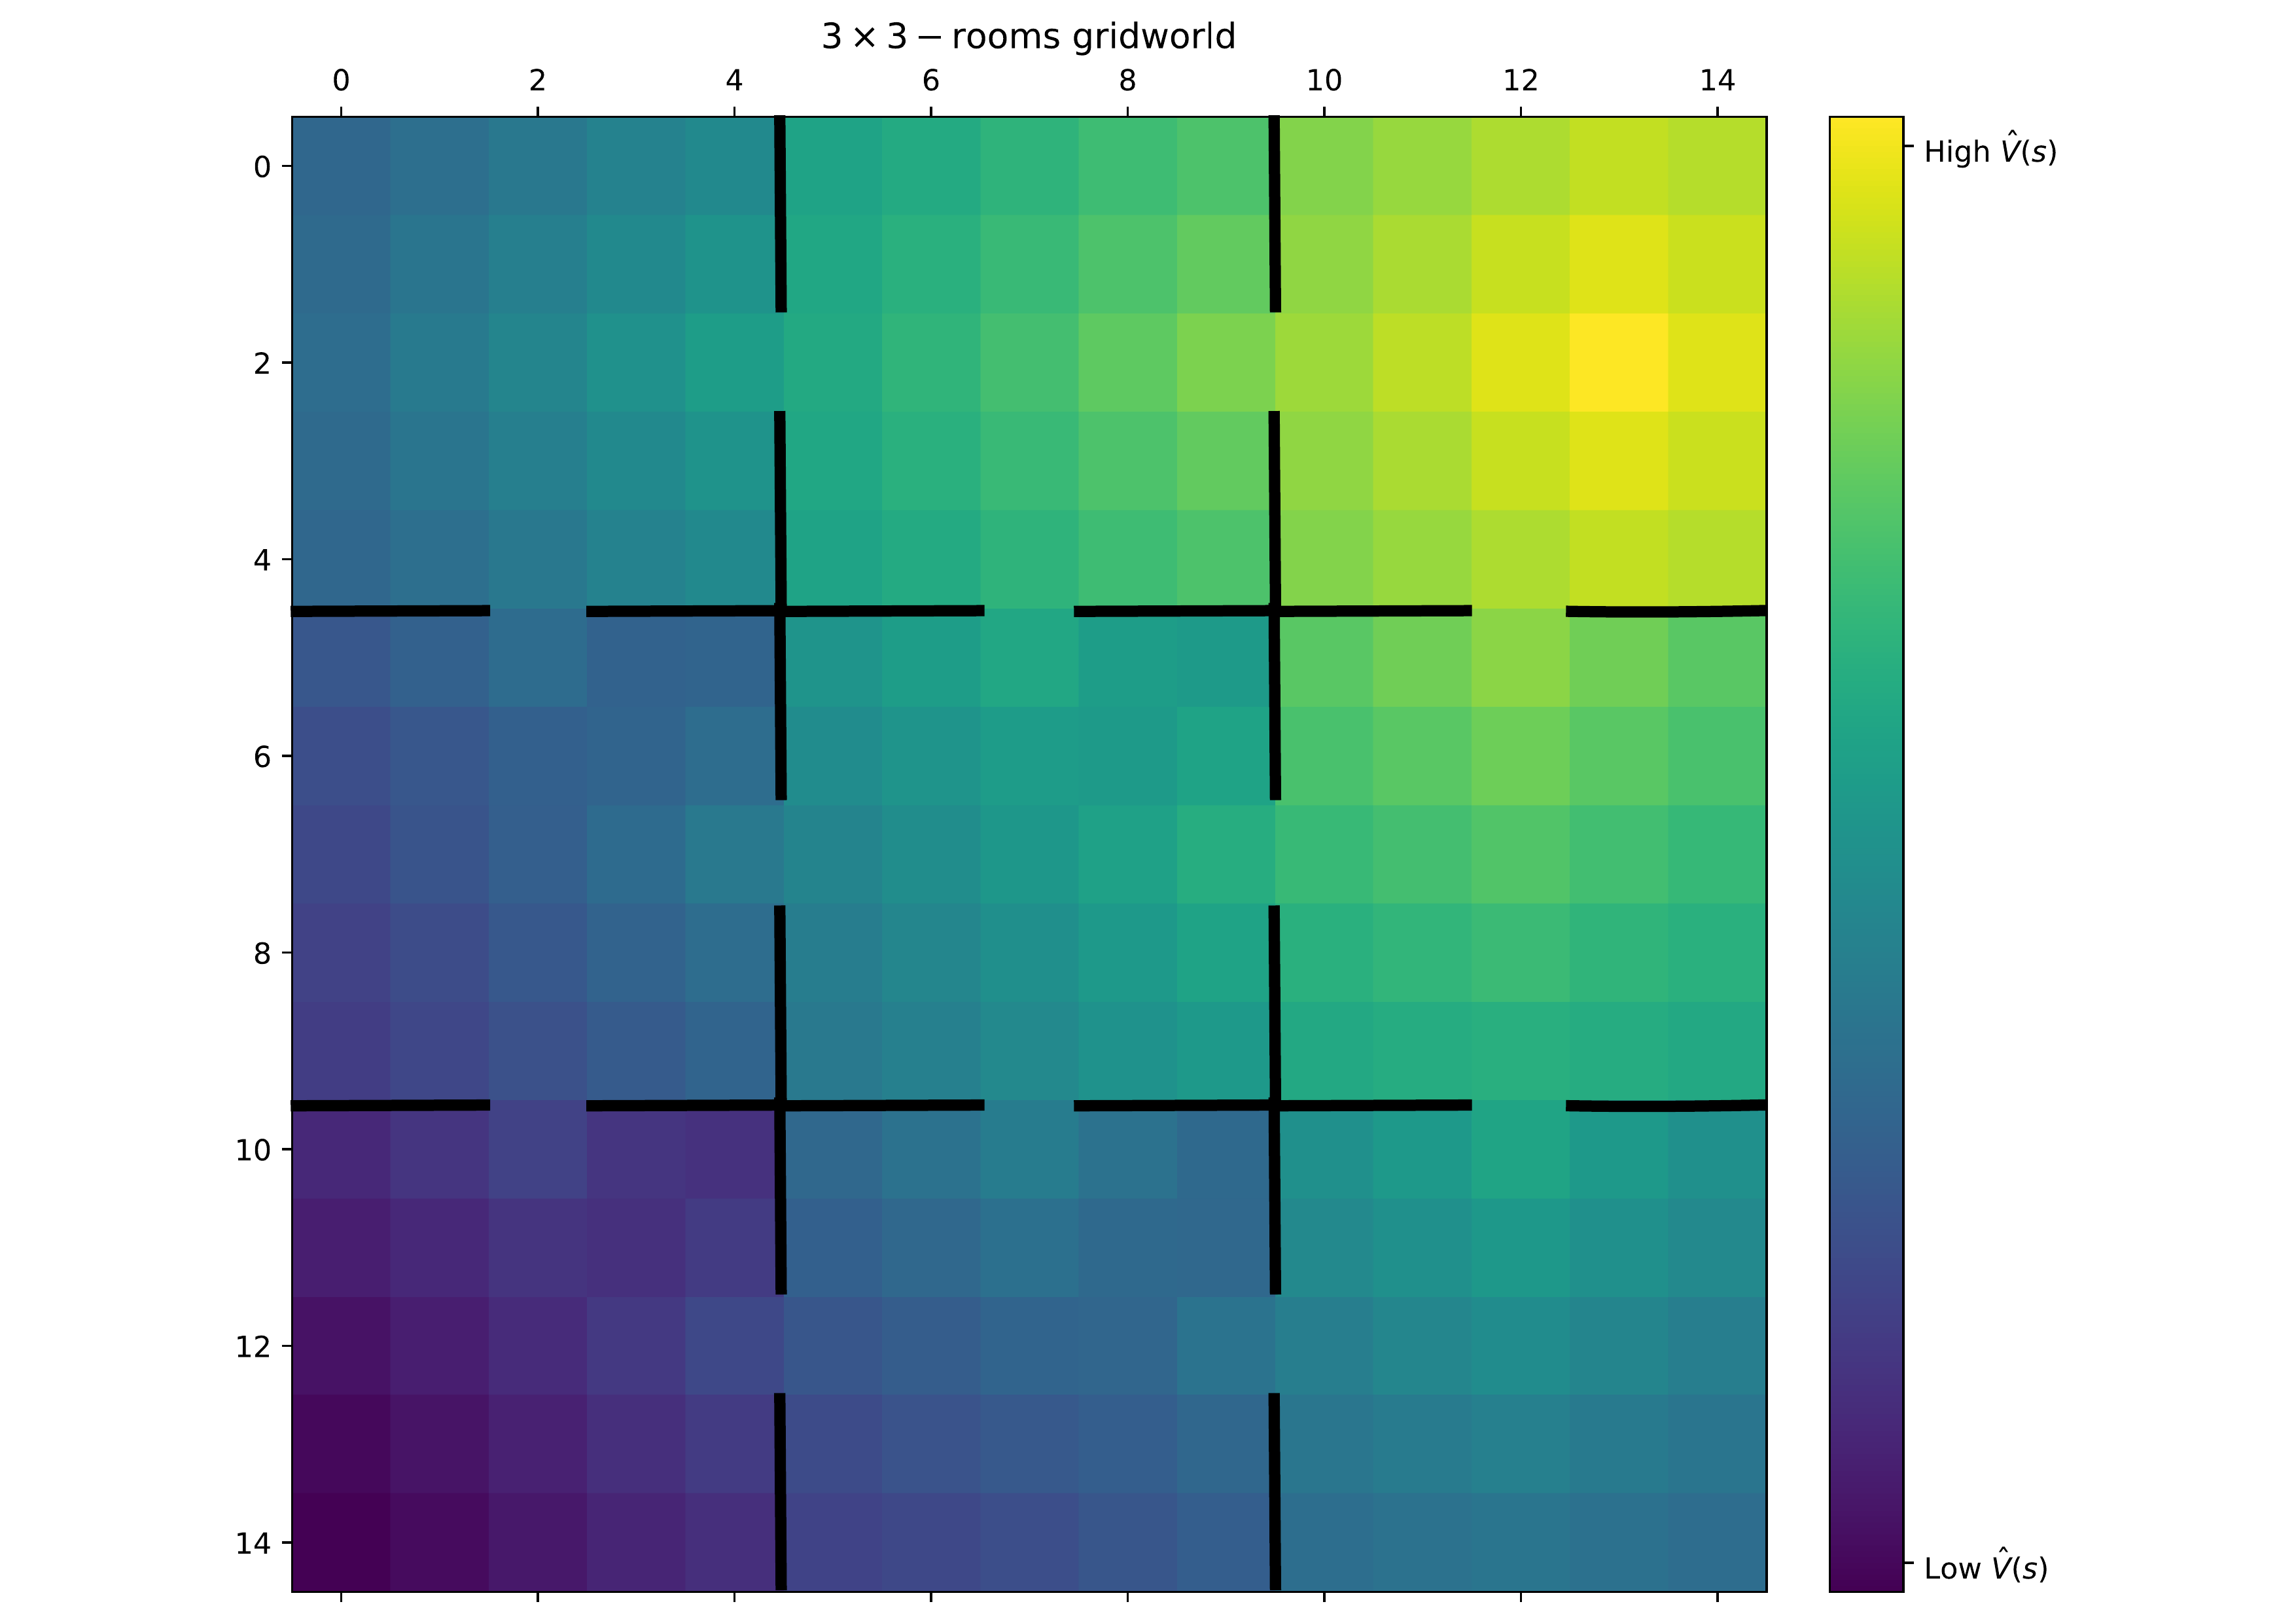
\includegraphics[scale=0.25]{Figures/grid_domain_VF.png}

\label{fig:vf_grid}
\end{figure}
    
\end{frame}


\begin{frame}{Experiments - Taxi domain}
    
    \begin{itemize}
    \item A passenger is located at one of the four corners and he must be carried to a certain corner (excluding the pickup location).
    \item Base LMDPs here are going to each of the corners.
    \item Sometimes there exist natural equivalence classes in facotres MDPs
\end{itemize}

    \begin{figure}[H]
    \centering
    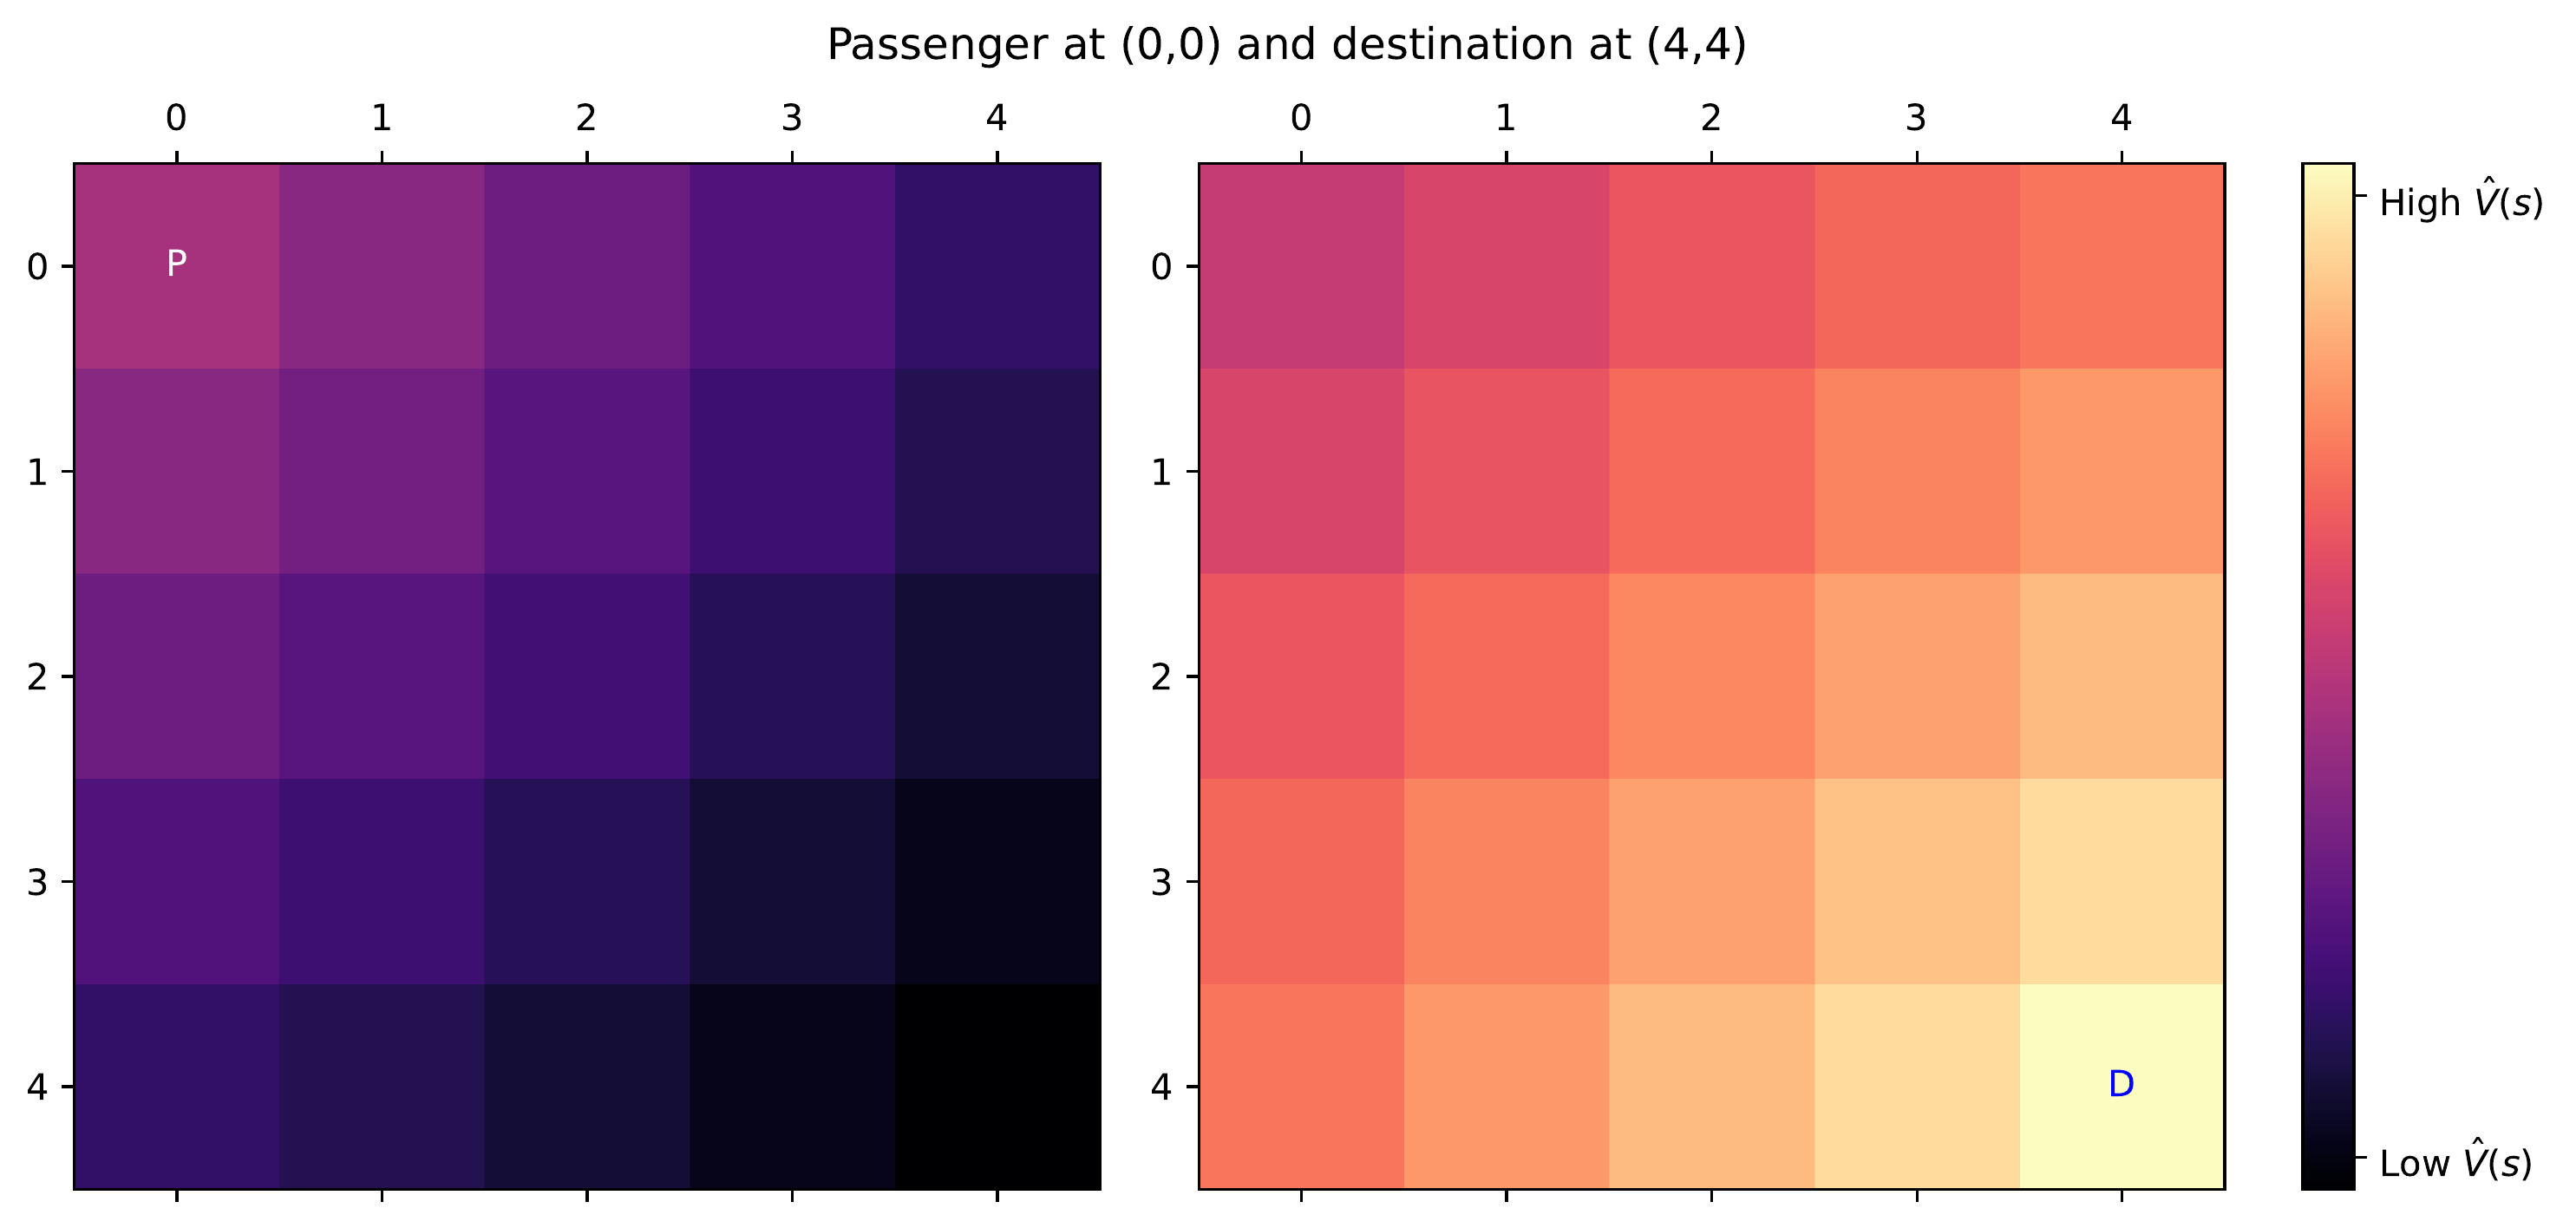
\includegraphics[scale=0.35]{Figures/taxi_dom_VF.png}
    
    \label{fig:vf_taxi}
    \end{figure}

\end{frame}


\section{Results}
\begin{frame}{Results - Rooms domain}

\begin{figure}[H]
\centering
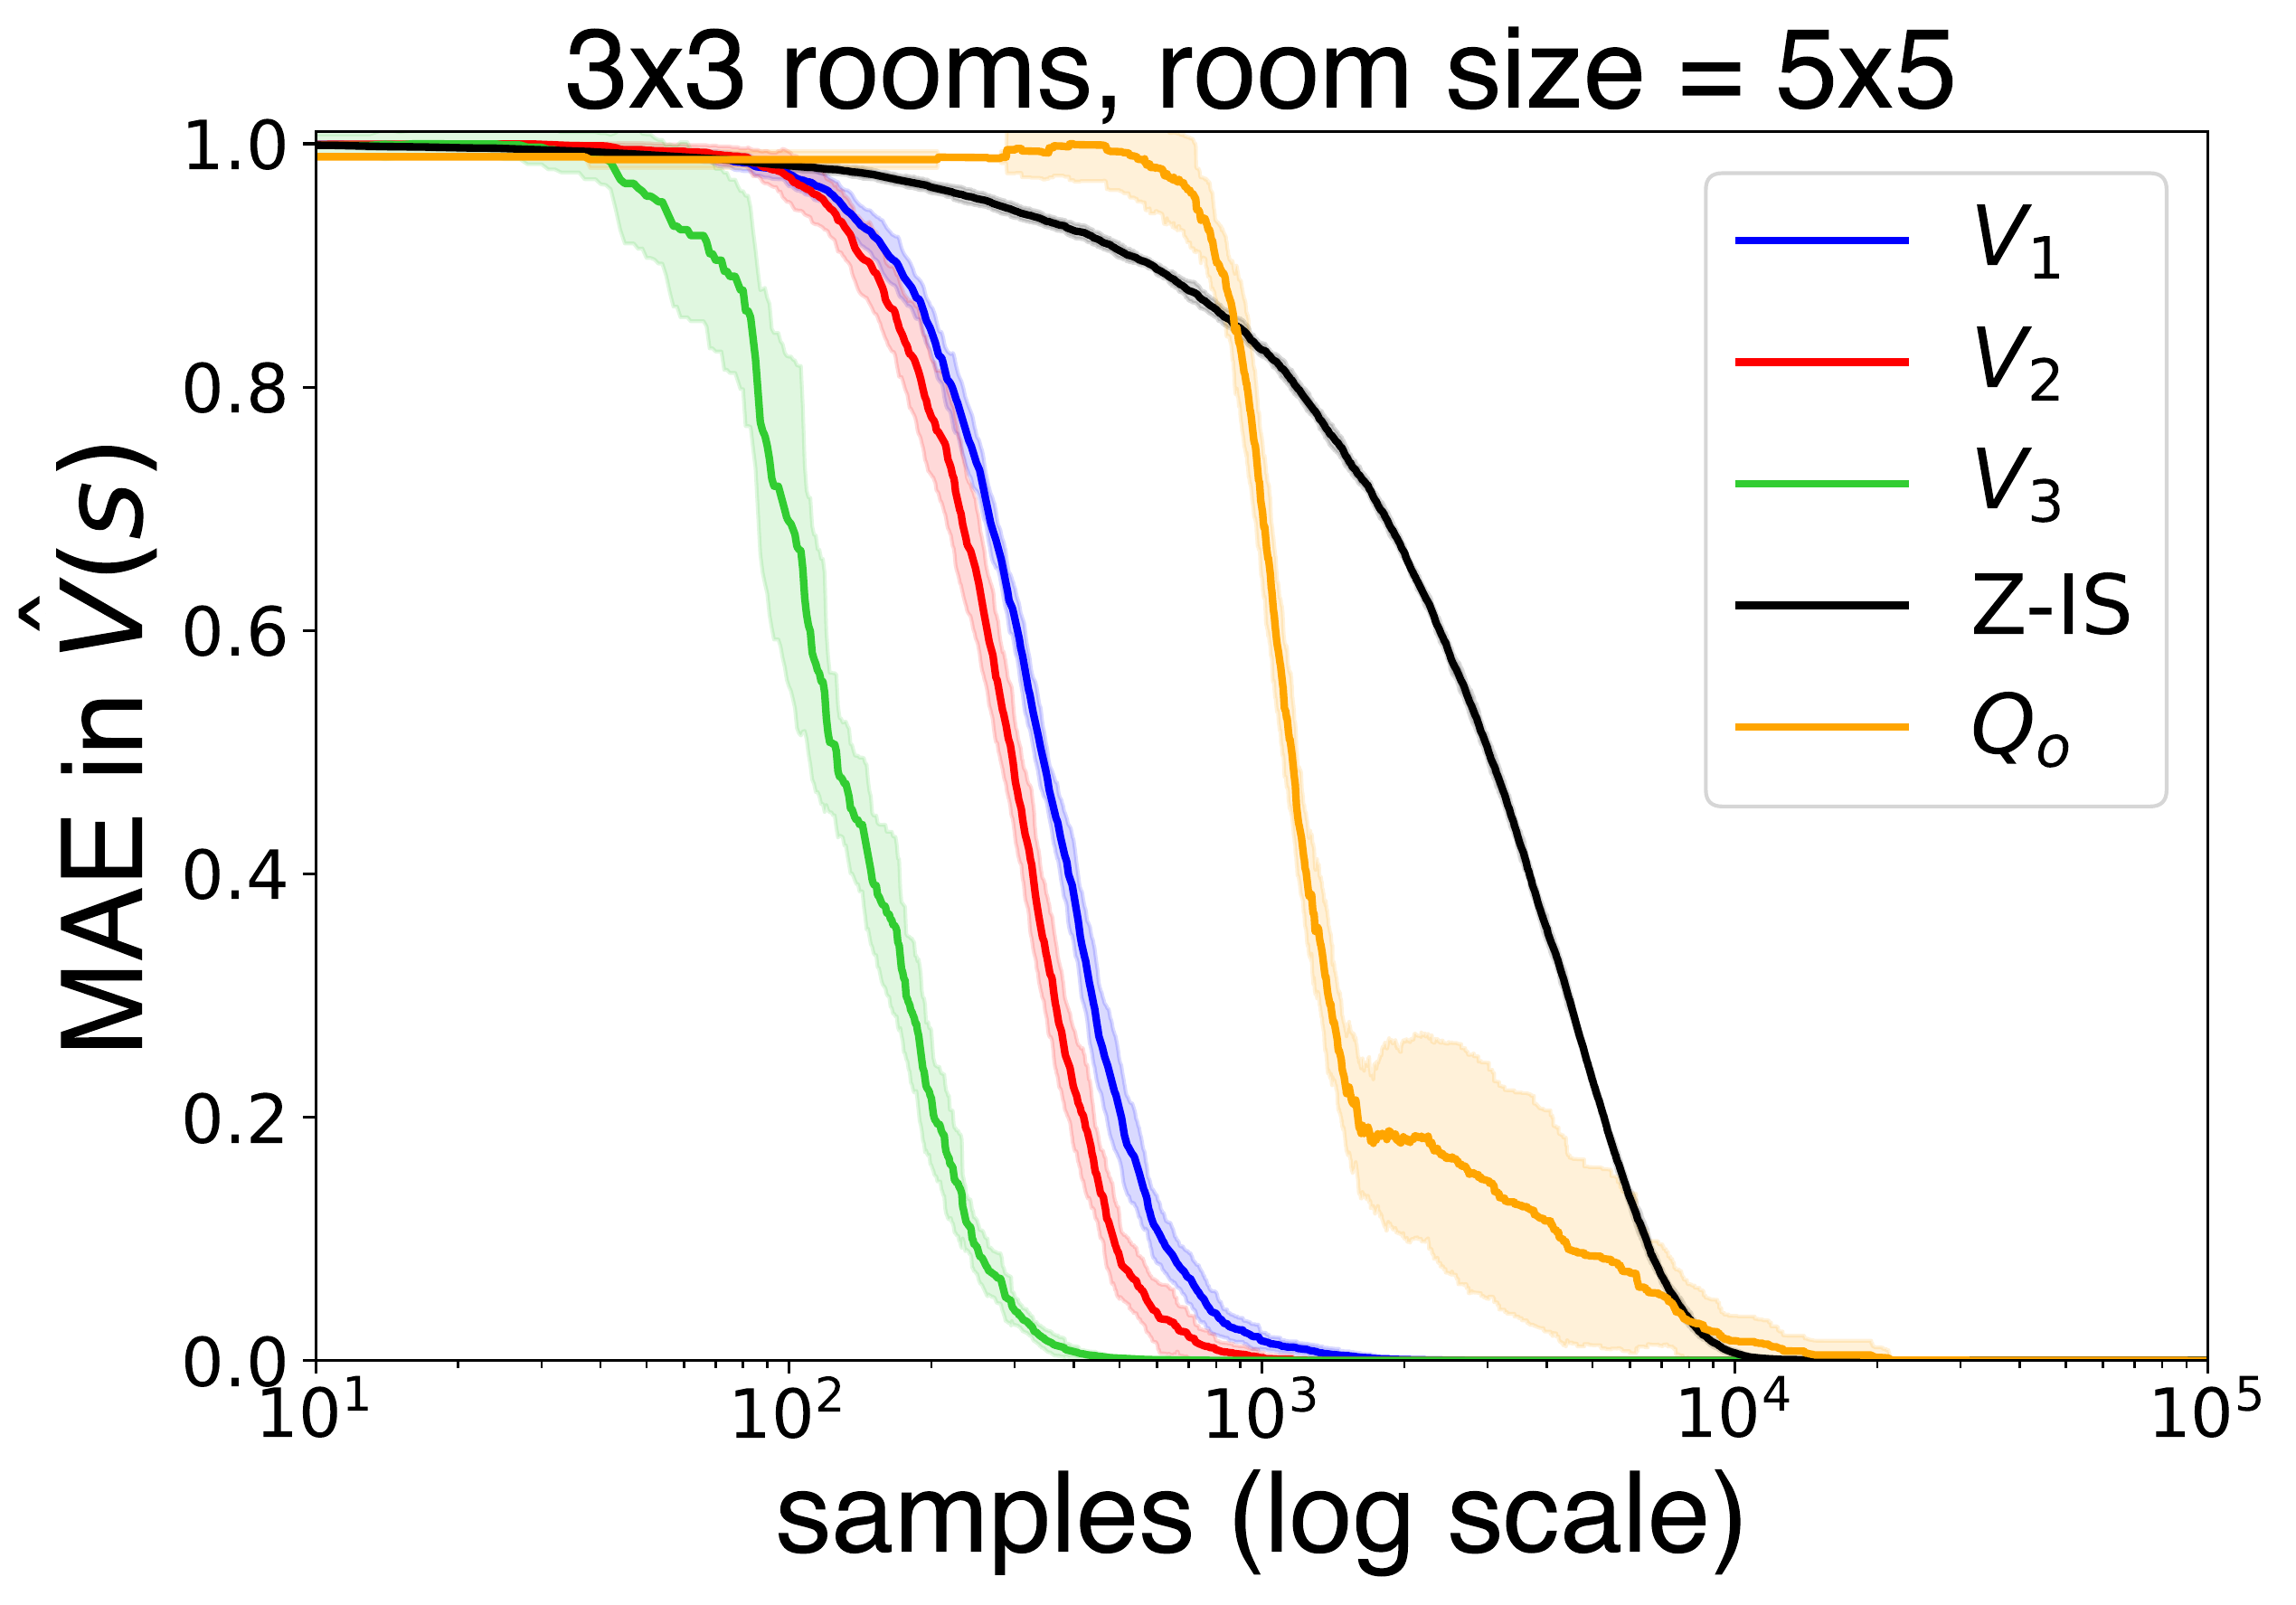
\includegraphics[scale=0.2]{Figures/nroom_3_3-1.png}
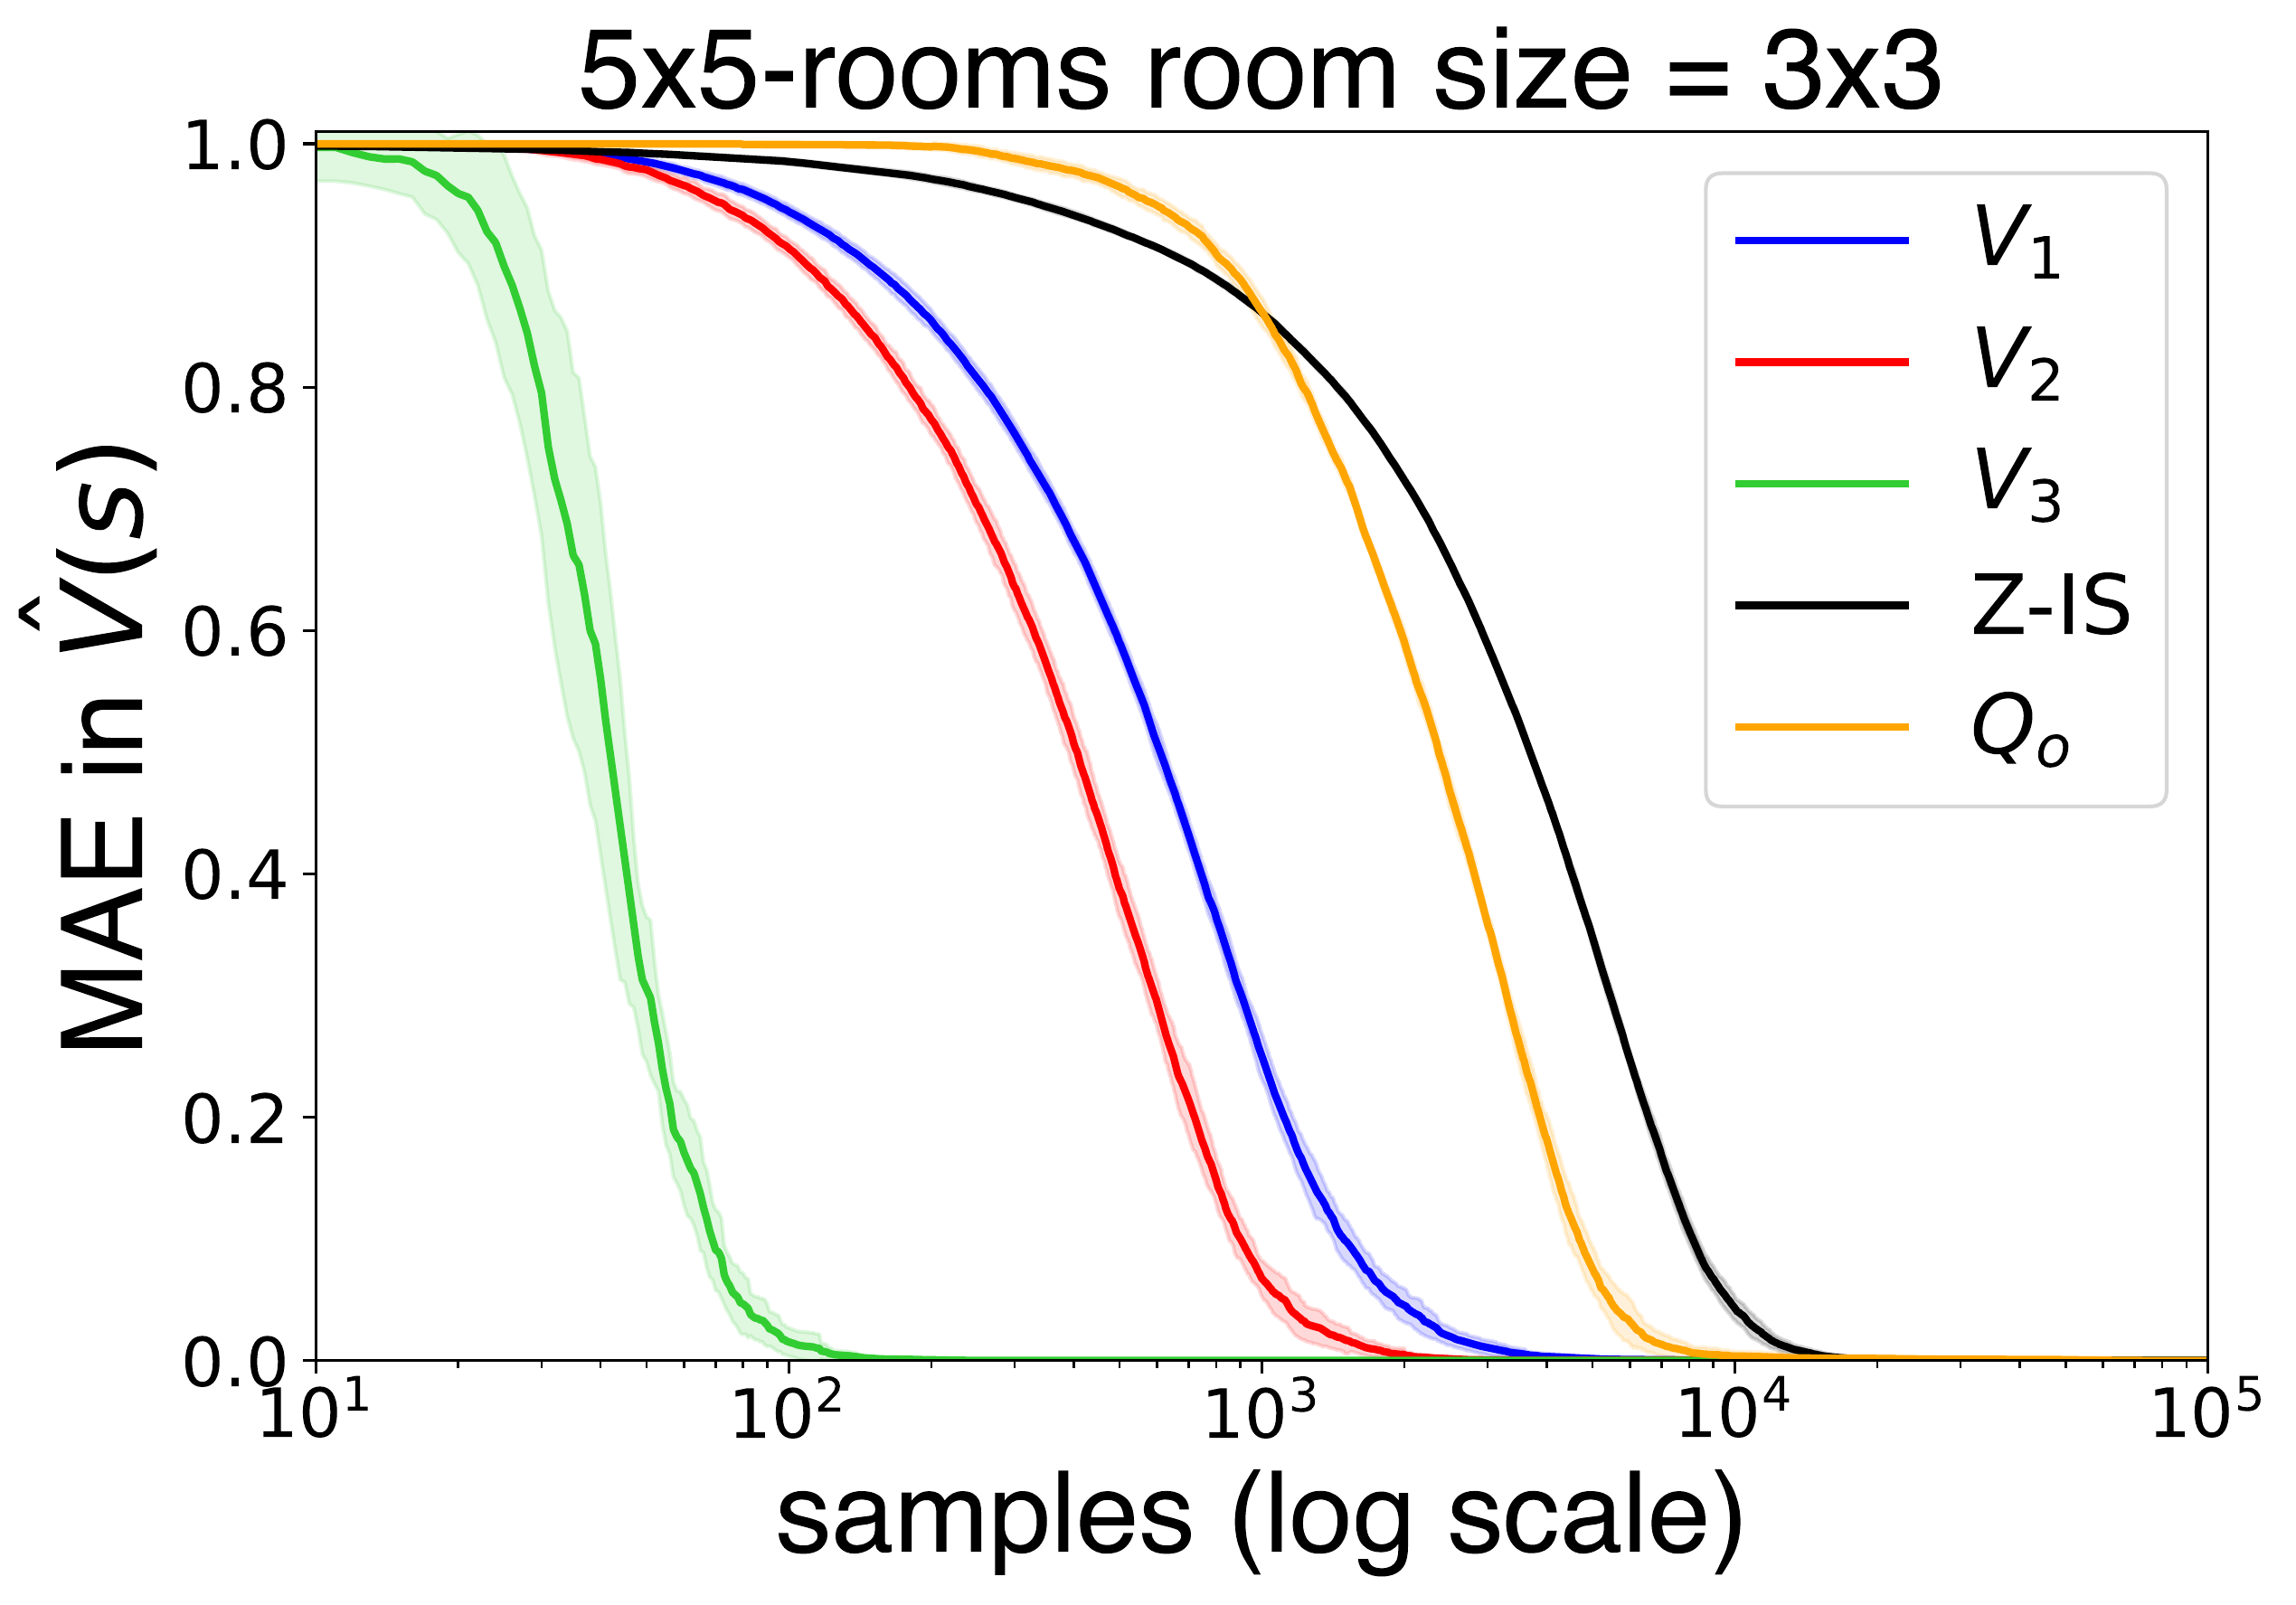
\includegraphics[scale=0.2]{Figures/nroom_5_5-1.png}
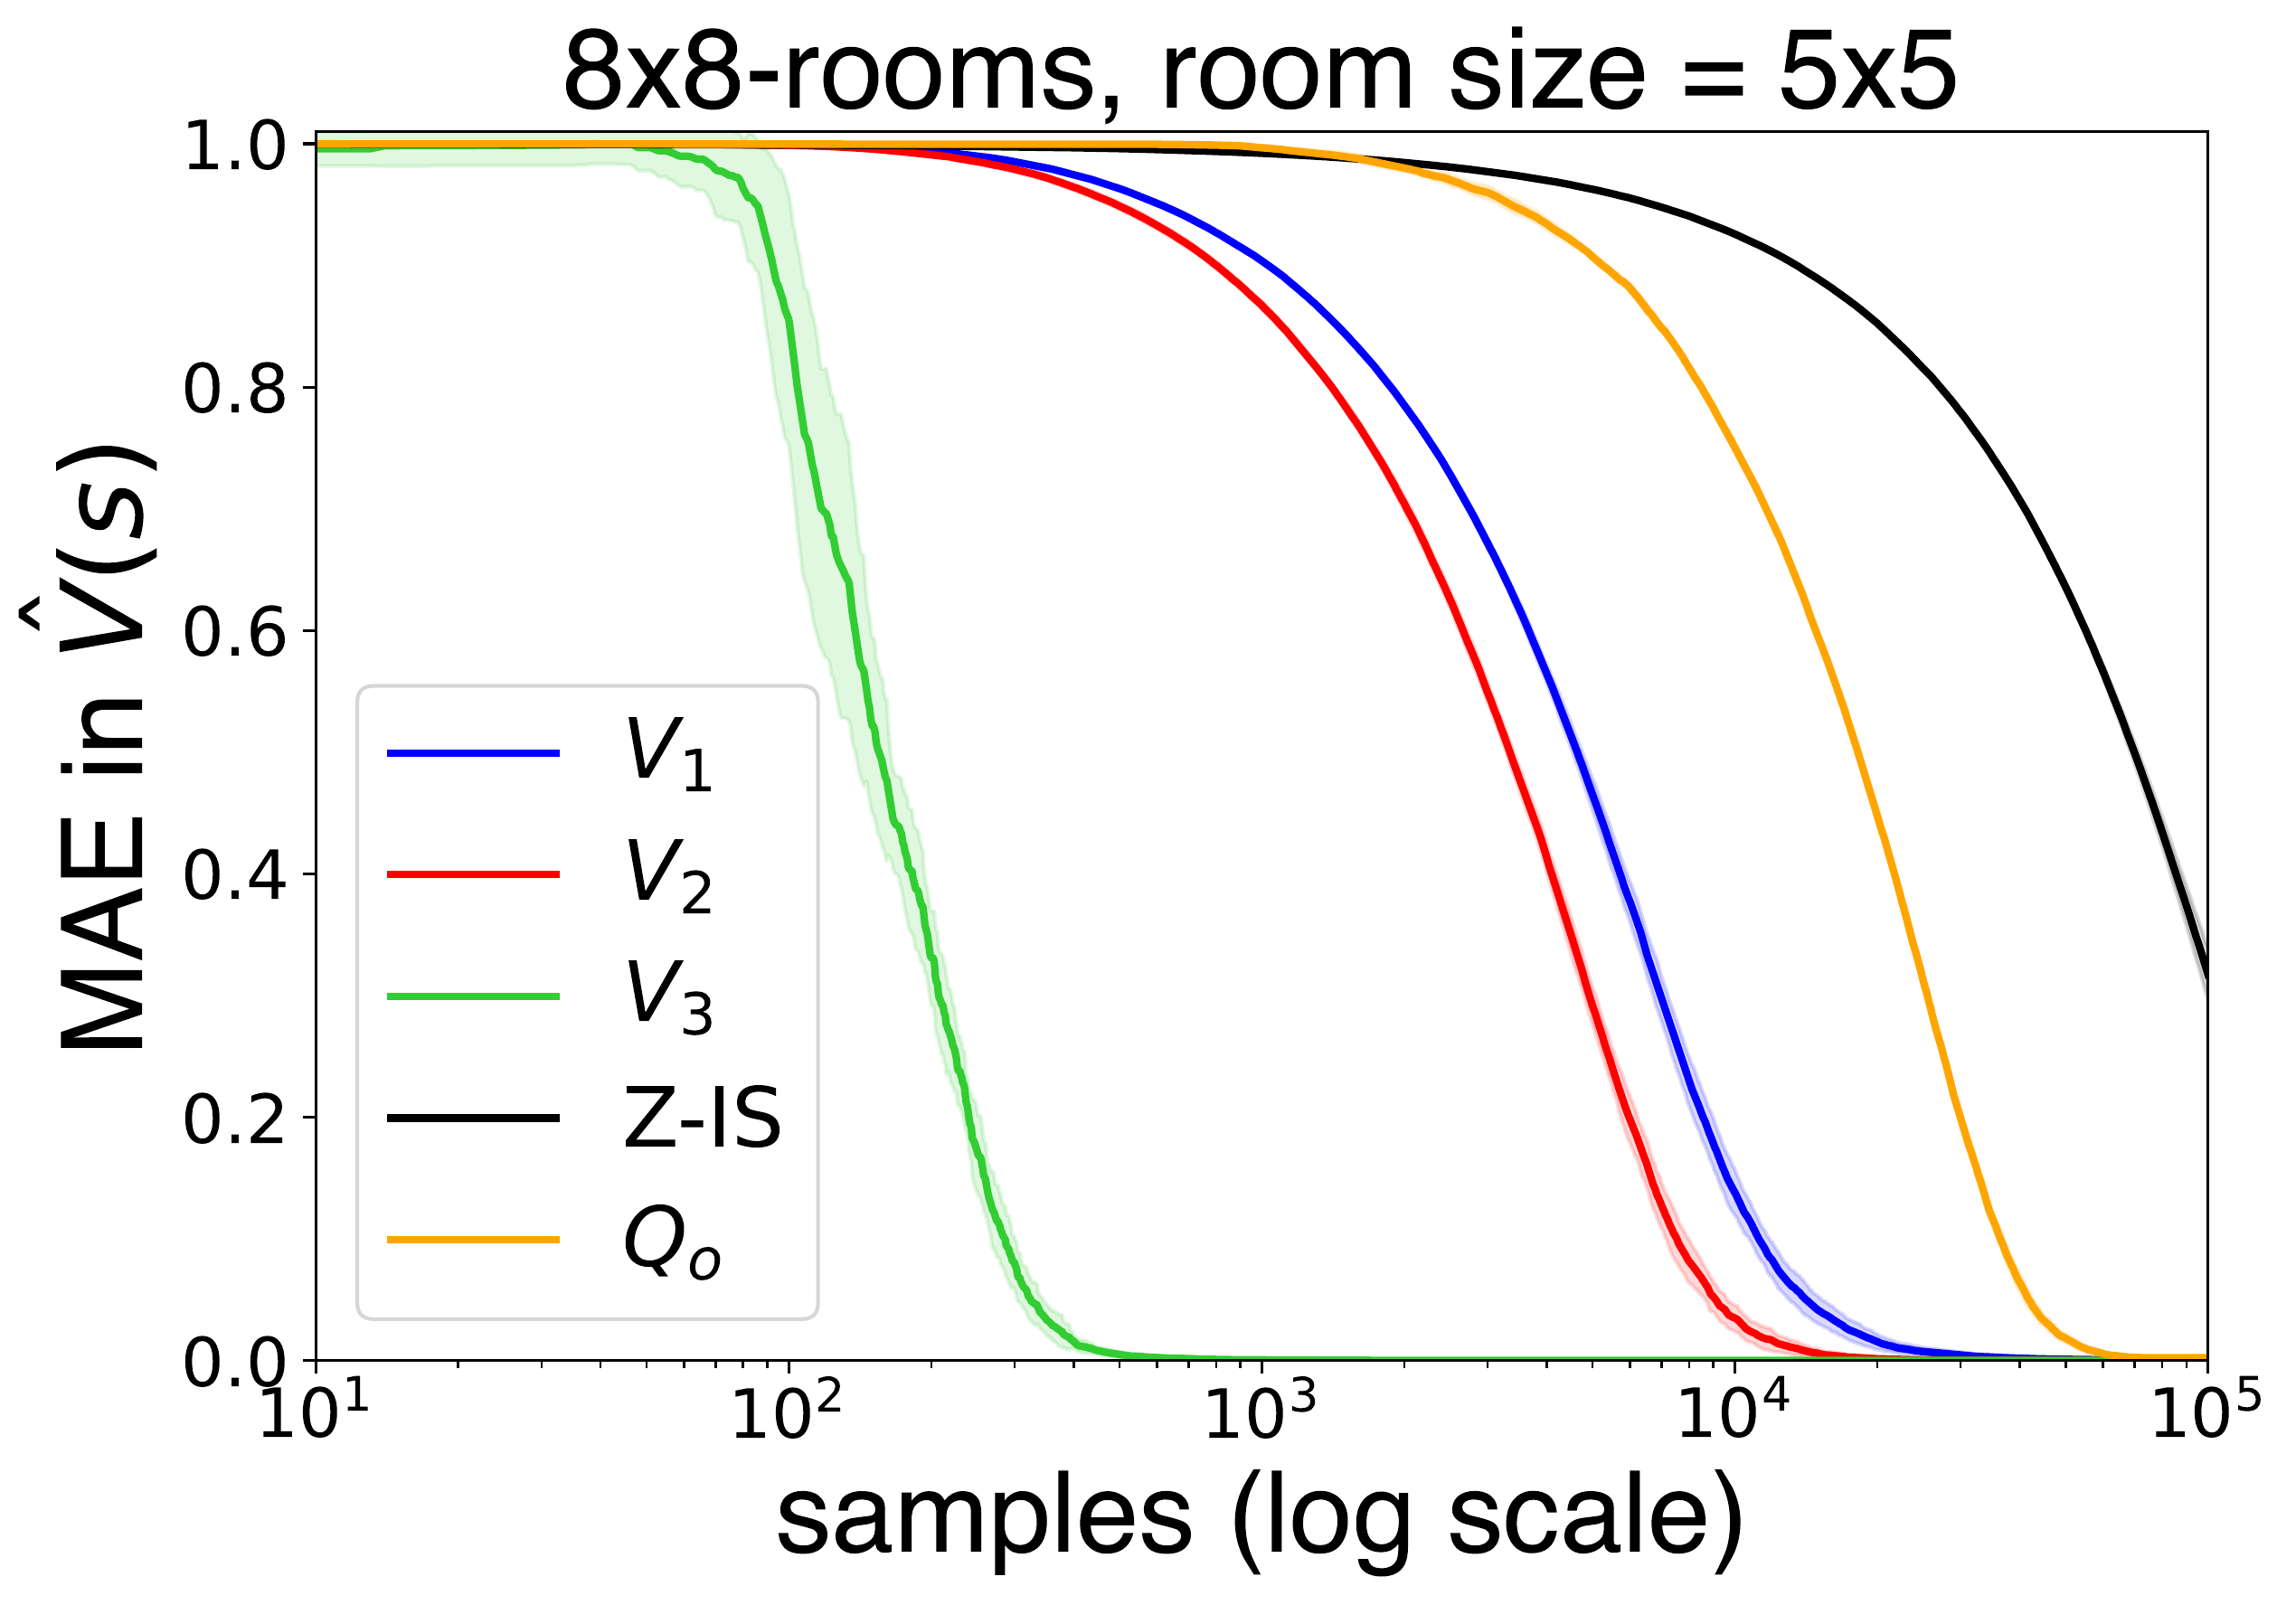
\includegraphics[scale=0.2]{Figures/nroom_8_8-1.png}

\caption{MAE over time for $3 \times 3$ (left), $5 \times 5$ (middle) and $8 \times 8$ (right) room instances.}
\label{fig:errors_grid}
\end{figure}

\end{frame}

\begin{frame}{Results - Taxi domain}

\begin{figure}[H]
\centering
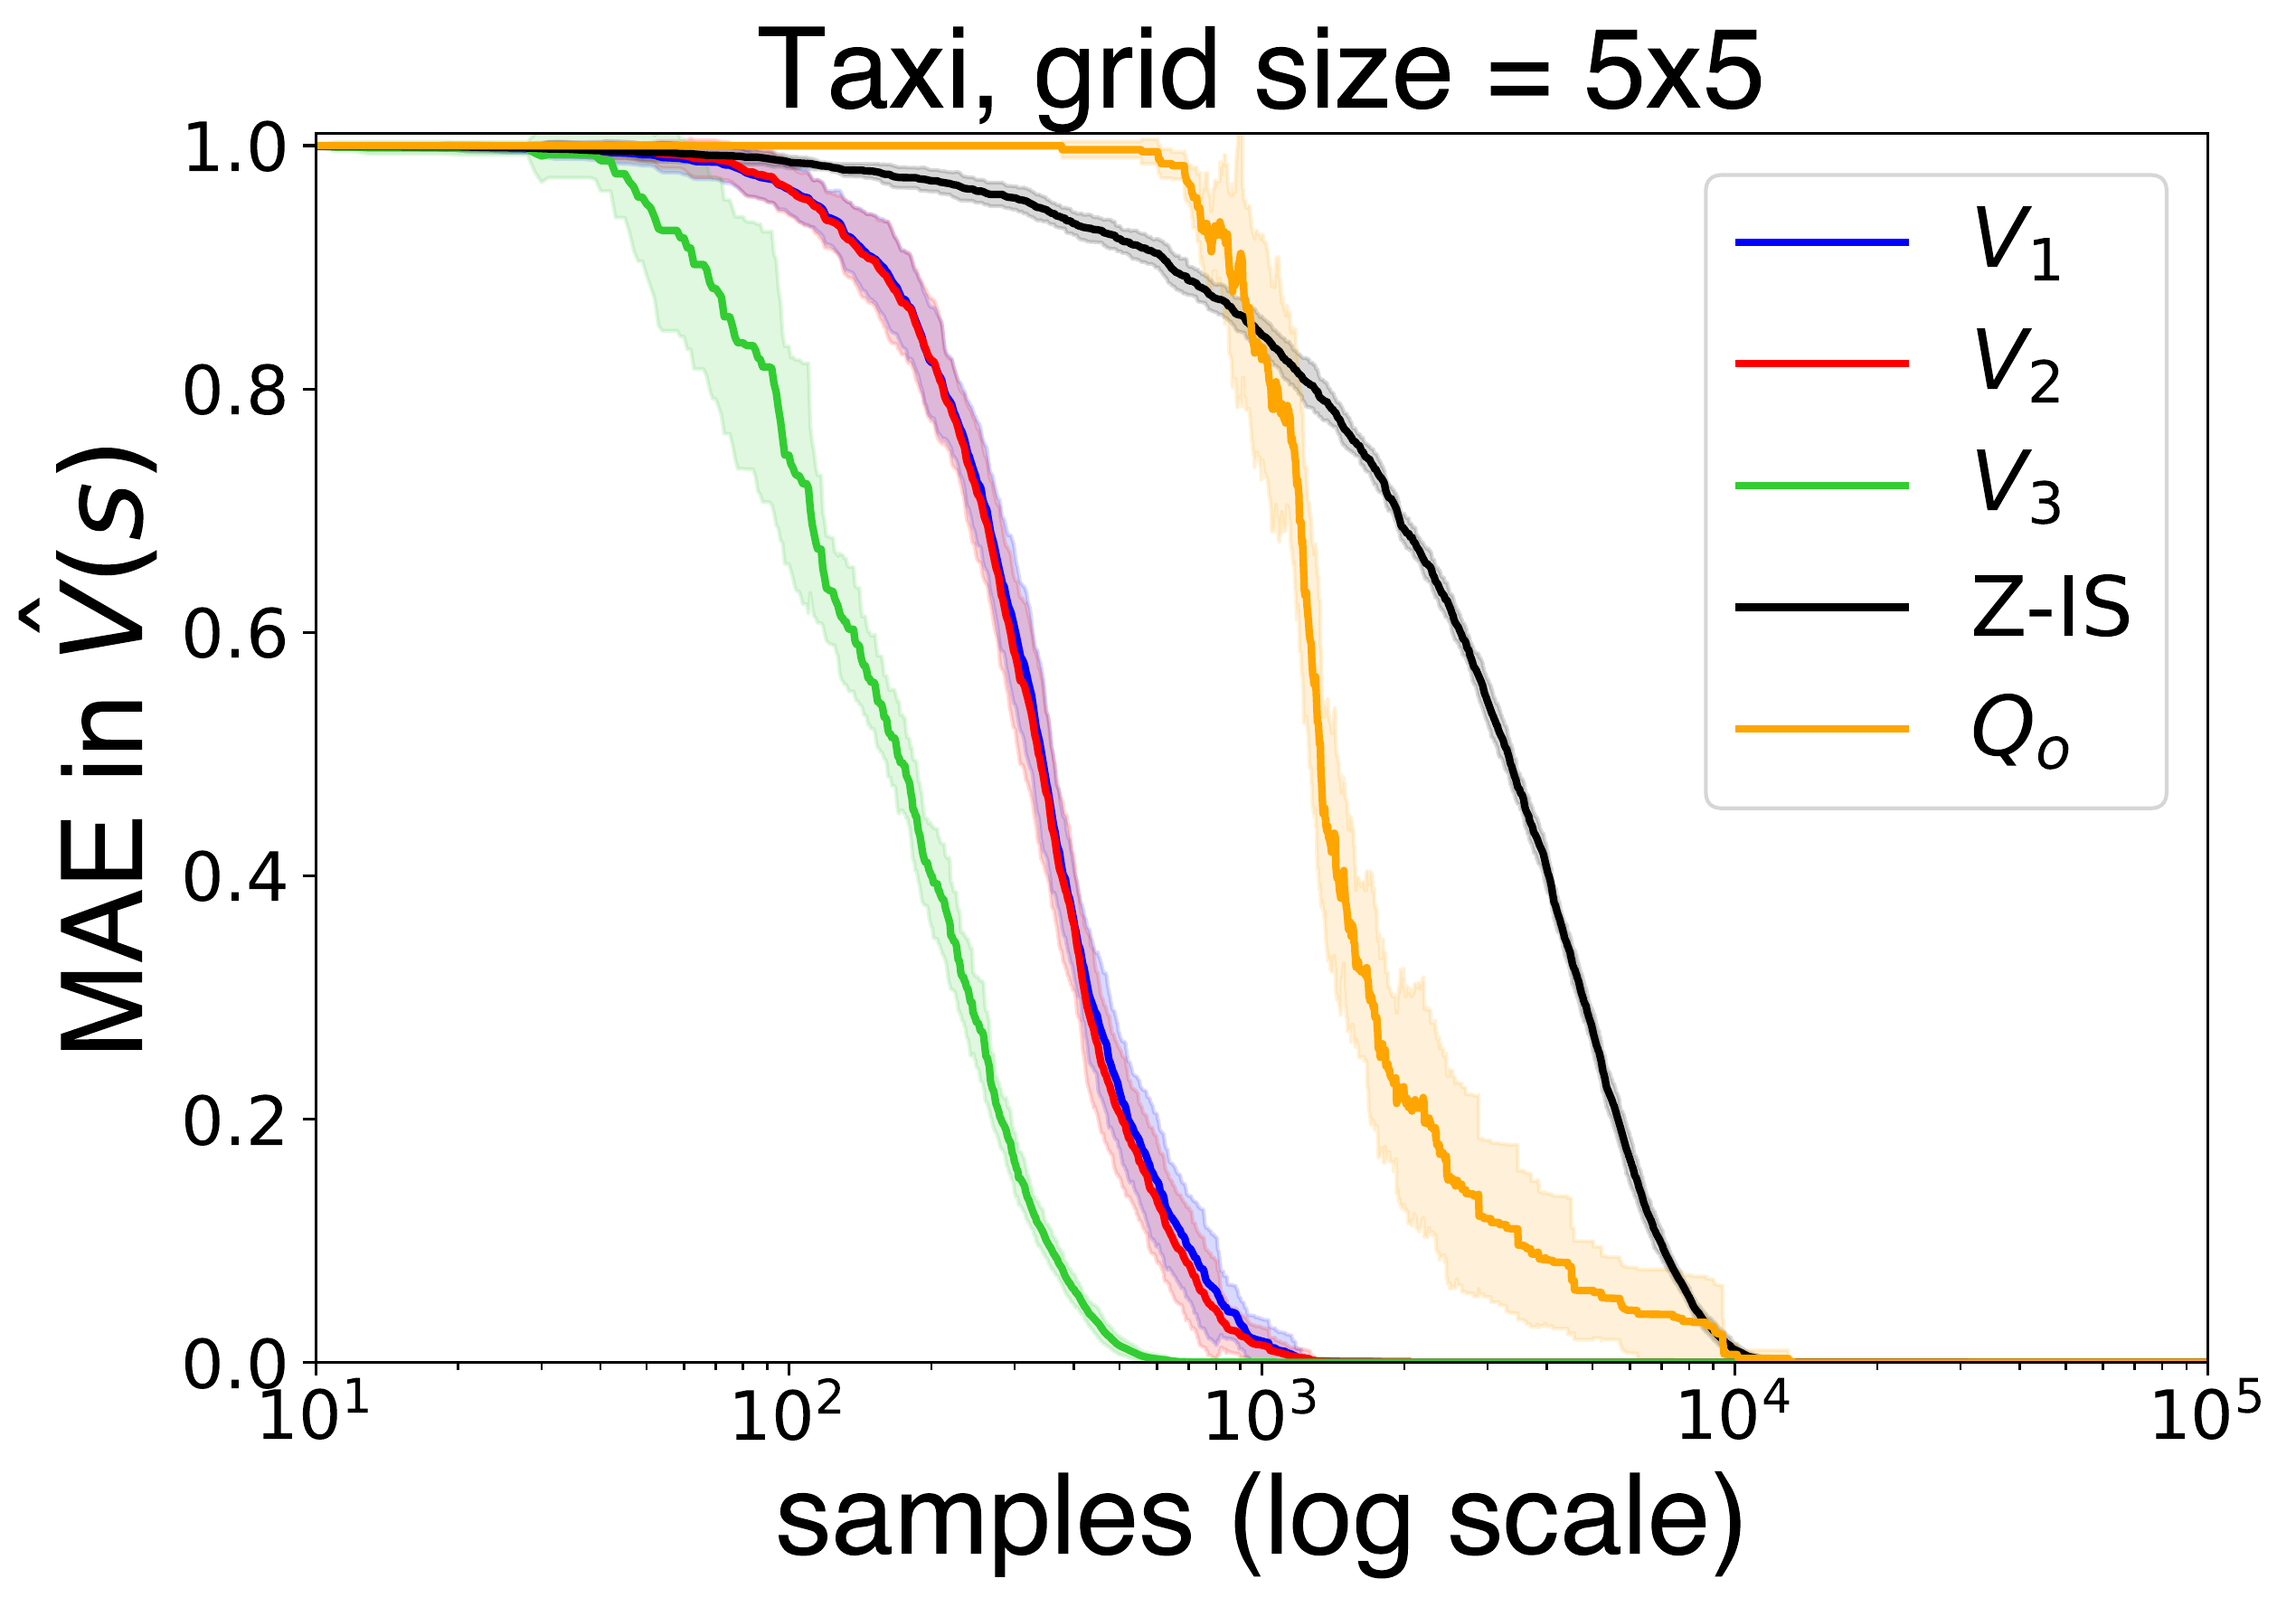
\includegraphics[scale=0.22]{Figures/taxi_5-1.png}
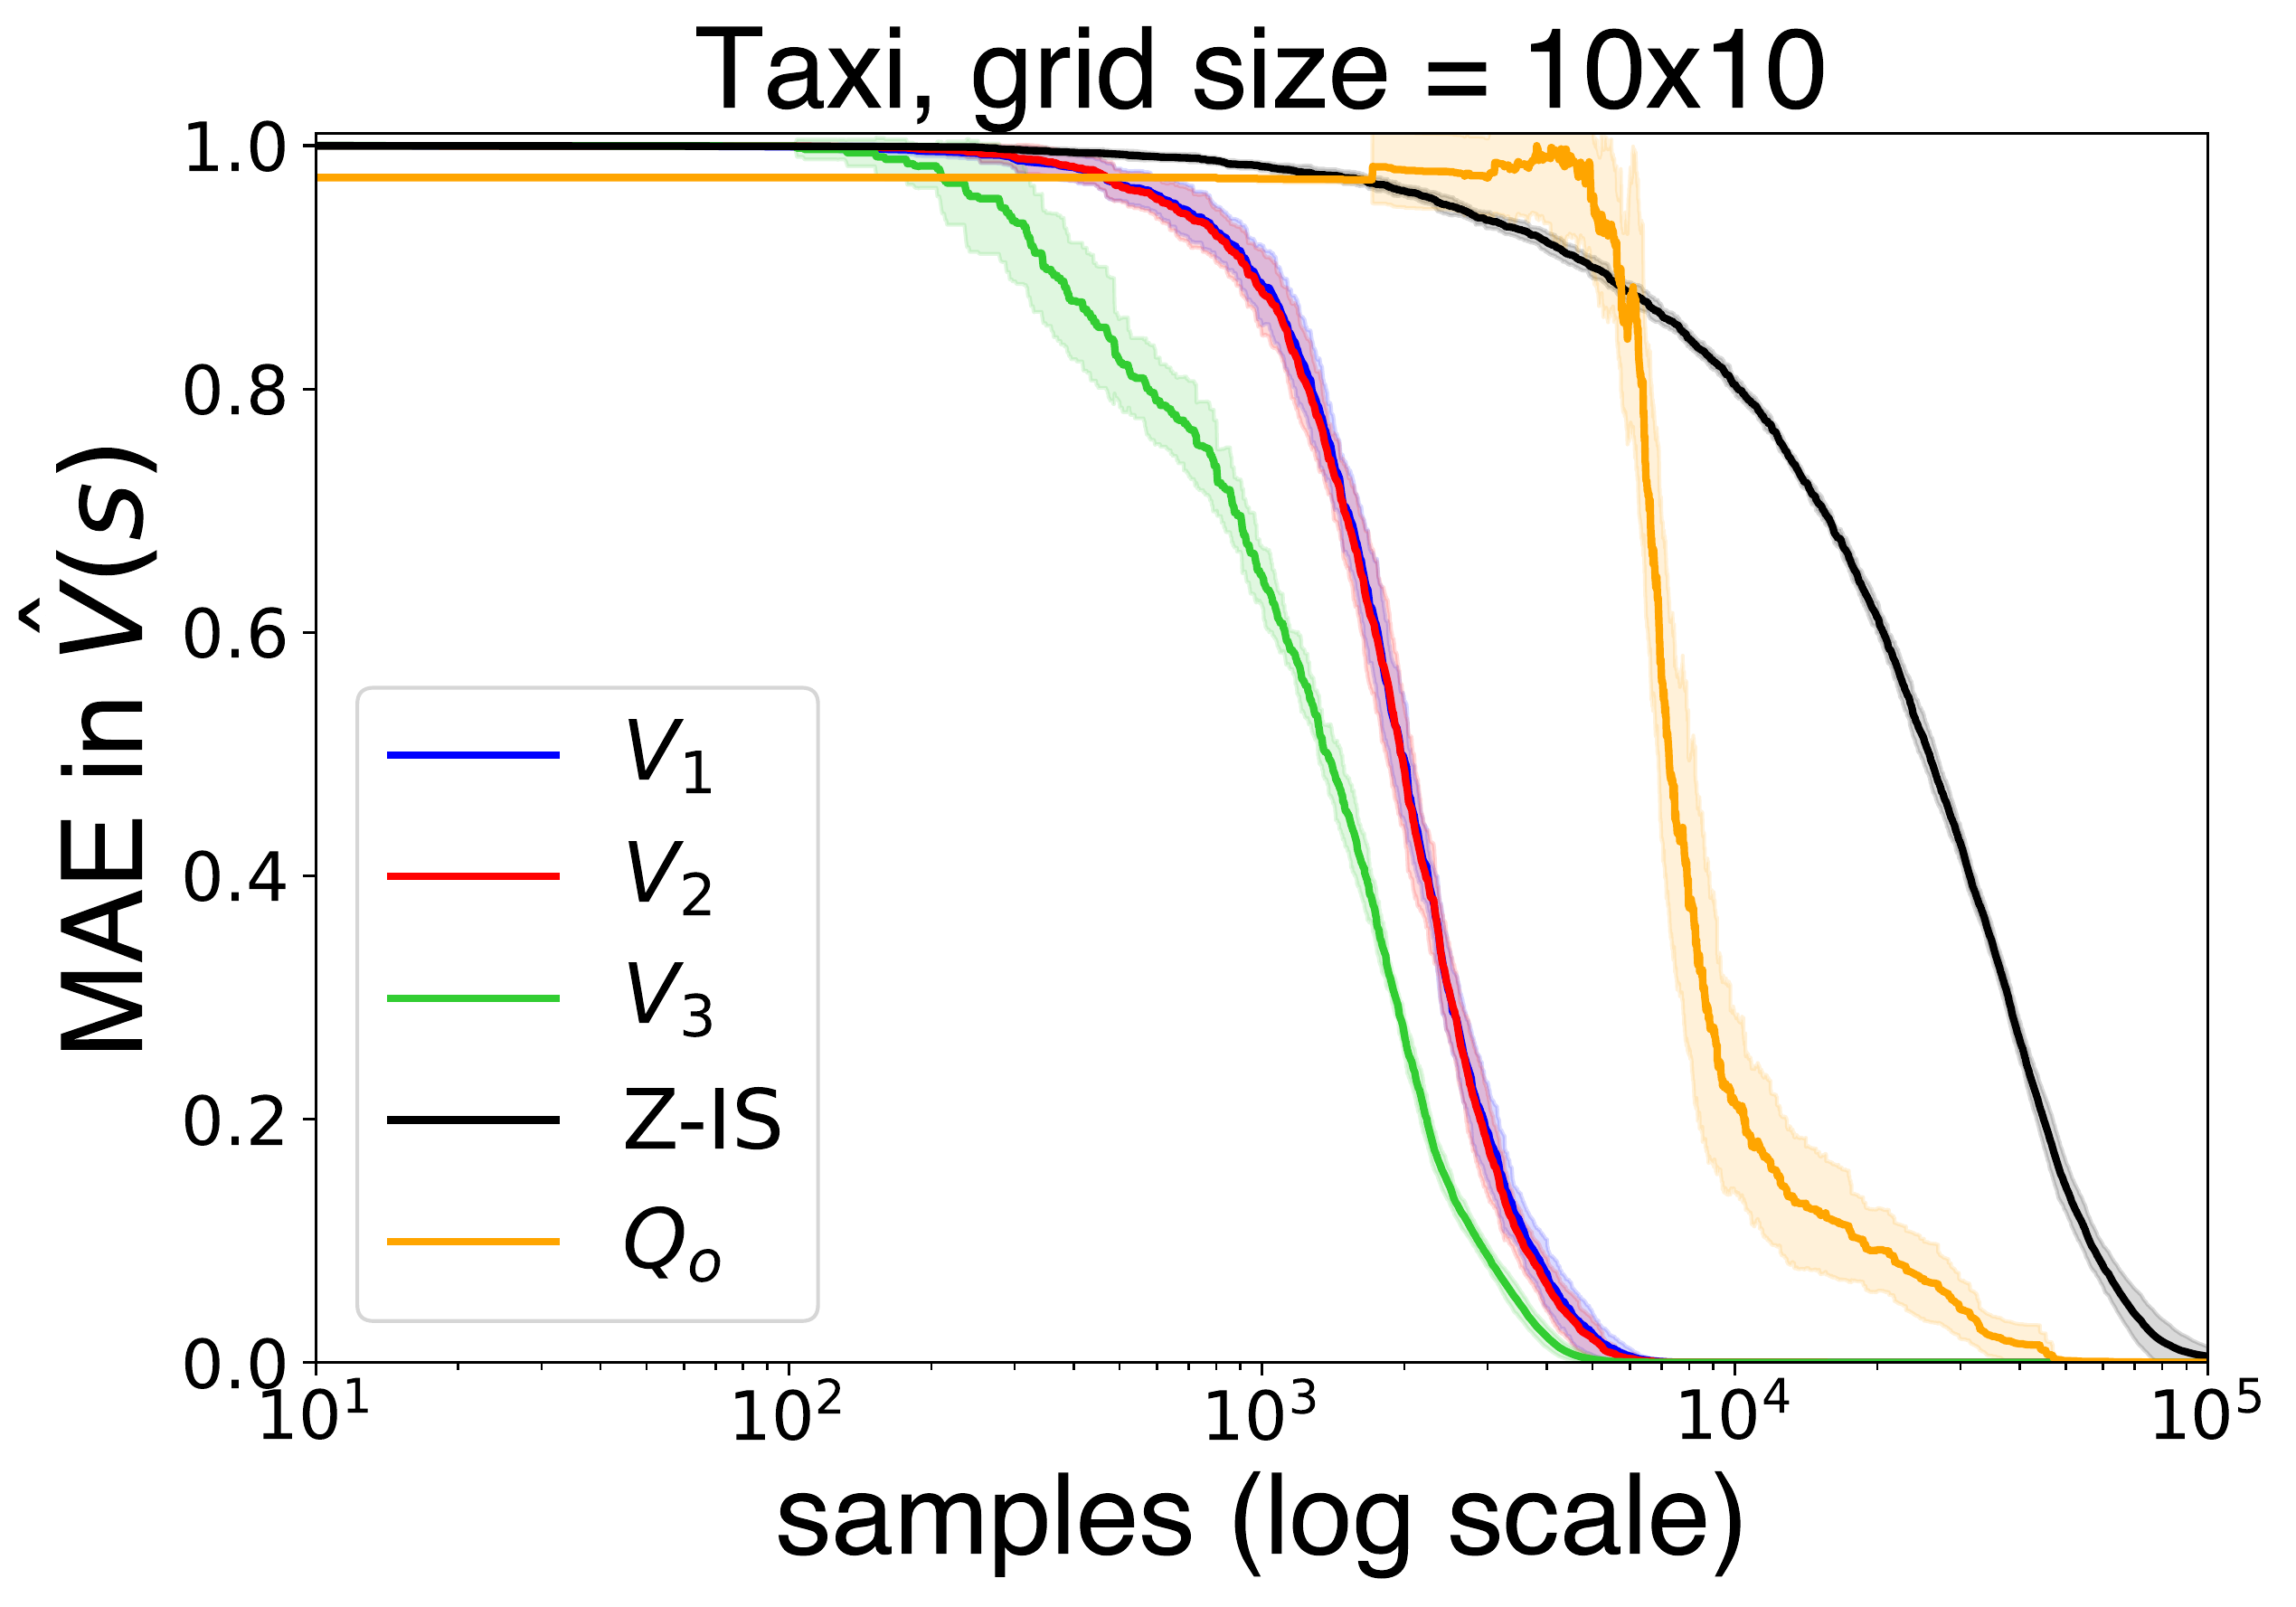
\includegraphics[scale=0.22]{Figures/taxi_10-1.png}
\caption{MAE over time for $5 \times 5$ (left) and $10 \times 10$ (right) grids of Taxi domain.}
\label{fig:errors_taxi}
\end{figure}

\end{frame}

\section{Contributions and Conclusion}
\begin{frame}{Contributions}
\begin{itemize}
    \item We define a novel scheme based on compositionality for solving subtasks. 
    \item The subtasks decomposition is at the level of the value function, thus our approach does not suffer from non-stationarity in the online setting. 
    \item Under mild assumptions, our method converges to the optimal value function.
    \item {\color{myred} In the options setting...}

\end{itemize}

\end{frame}

\begin{frame}{Conclusion}

Unlike typical HRL approaches, we no longer need a high-level policy that selects among subgoals (e.g. non-stationarity in SMDPs). Instead, we are able to retrieve the optimal value function for each state thanks to the decomposition of the value function in terms of the values of base LMDPs.
    
\end{frame}


\begin{frame}[allowframebreaks]{}
    \bibliographystyle{plain}
    \bibliography{references}
\end{frame}

\end{document}
References